\documentclass[journal,12pt,twocolumn]{IEEEtran}
%
\usepackage{setspace}
\usepackage{gensymb}
\usepackage{xcolor}
\usepackage{caption}
%\usepackage{subcaption}
%\doublespacing
\singlespacing
\usepackage{multicol}

\usepackage{iithtlc}
%\usepackage{graphicx}
%\usepackage{amssymb}
%\usepackage{relsize}
\usepackage[cmex10]{amsmath}
\usepackage{mathtools}
%\usepackage{amsthm}
%\interdisplaylinepenalty=2500
%\savesymbol{iint}
%\usepackage{txfonts}
%\restoresymbol{TXF}{iint}
%\usepackage{wasysym}
\usepackage{amsthm}
\usepackage{mathrsfs}
\usepackage{txfonts}
\usepackage{stfloats}
\usepackage{cite}
\usepackage{cases}
\usepackage{subfig}
%\usepackage{xtab}
\usepackage{longtable}
\usepackage{multirow}
%\usepackage{algorithm}
%\usepackage{algpseudocode}
\usepackage{enumitem}
\usepackage{mathtools}
%\usepackage{stmaryrd}

\usepackage{listings}
    \usepackage[latin1]{inputenc}                                 %%
    \usepackage{color}                                            %%
    \usepackage{array}                                            %%
    \usepackage{longtable}                                        %%
    \usepackage{calc}                                             %%
    \usepackage{multirow}                                         %%
    \usepackage{hhline}                                           %%
    \usepackage{ifthen}                                           %%
  %optionally (for landscape tables embedded in another document): %%
    \usepackage{lscape}     

%\usepackage{wasysym}
%\newcounter{MYtempeqncnt}
\DeclareMathOperator*{\Res}{Res}
%\renewcommand{\baselinestretch}{2}
\renewcommand\thesection{\arabic{section}}
\renewcommand\thesubsection{\thesection.\arabic{subsection}}
\renewcommand\thesubsubsection{\thesubsection.\arabic{subsubsection}}

\renewcommand\thesectiondis{\arabic{section}}
\renewcommand\thesubsectiondis{\thesectiondis.\arabic{subsection}}
\renewcommand\thesubsubsectiondis{\thesubsectiondis.\arabic{subsubsection}}

% correct bad hyphenation here
\hyphenation{op-tical net-works semi-conduc-tor}

\def\inputGnumericTable{}  

\lstset{
language=python,
frame=single, 
breaklines=true
}

\begin{document}
%

\theoremstyle{definition}

\newtheorem{theorem}{Theorem}[section]
\newtheorem{problem}{Problem}
\newtheorem{proposition}{Proposition}[section]
\newtheorem{lemma}{Lemma}[section]
\newtheorem{corollary}[theorem]{Corollary}
\newtheorem{example}{Example}[section]
\newtheorem{definition}{Definition}[section]
%\newtheorem{algorithm}{Algorithm}[section]
%\newtheorem{cor}{Corollary}
\newcommand{\BEQA}{\begin{eqnarray}}
\newcommand{\EEQA}{\end{eqnarray}}
\newcommand{\define}{\stackrel{\triangle}{=}}

\bibliographystyle{IEEEtran}
%\bibliographystyle{ieeetr}



\providecommand{\pr}[1]{\ensuremath{\Pr\left(#1\right)}}
\providecommand{\qfunc}[1]{\ensuremath{Q\left(#1\right)}}
\providecommand{\sbrak}[1]{\ensuremath{{}\left[#1\right]}}
\providecommand{\lsbrak}[1]{\ensuremath{{}\left[#1\right.}}
\providecommand{\rsbrak}[1]{\ensuremath{{}\left.#1\right]}}
\providecommand{\brak}[1]{\ensuremath{\left(#1\right)}}
\providecommand{\lbrak}[1]{\ensuremath{\left(#1\right.}}
\providecommand{\rbrak}[1]{\ensuremath{\left.#1\right)}}
\providecommand{\cbrak}[1]{\ensuremath{\left\{#1\right\}}}
\providecommand{\lcbrak}[1]{\ensuremath{\left\{#1\right.}}
\providecommand{\rcbrak}[1]{\ensuremath{\left.#1\right\}}}
\theoremstyle{remark}
\newtheorem{rem}{Remark}
\newcommand{\sgn}{\mathop{\mathrm{sgn}}}
\providecommand{\abs}[1]{\left\vert#1\right\vert}
\providecommand{\res}[1]{\Res\displaylimits_{#1}} 
\providecommand{\norm}[1]{\lVert#1\rVert}
\providecommand{\mtx}[1]{\mathbf{#1}}
\providecommand{\mean}[1]{E\left[ #1 \right]}
\providecommand{\fourier}{\overset{\mathcal{F}}{ \rightleftharpoons}}
%\providecommand{\hilbert}{\overset{\mathcal{H}}{ \rightleftharpoons}}
\providecommand{\system}{\overset{\mathcal{H}}{ \longleftrightarrow}}
\providecommand{\gauss}[2]{\mathcal{N}\ensuremath{\left(#1,#2\right)}}
	%\newcommand{\solution}[2]{\textbf{Solution:}{#1}}
\newcommand{\solution}{\noindent \textbf{Solution: }}
\providecommand{\dec}[2]{\ensuremath{\overset{#1}{\underset{#2}{\gtrless}}}}
%\numberwithin{equation}{section}
%\numberwithin{problem}{section}

\def\putbox#1#2#3{\makebox[0in][l]{\makebox[#1][l]{}\raisebox{\baselineskip}[0in][0in]{\raisebox{#2}[0in][0in]{#3}}}}
     \def\rightbox#1{\makebox[0in][r]{#1}}
     \def\centbox#1{\makebox[0in]{#1}}
     \def\topbox#1{\raisebox{-\baselineskip}[0in][0in]{#1}}
     \def\midbox#1{\raisebox{-0.5\baselineskip}[0in][0in]{#1}}


% paper title
% can use linebreaks \\ within to get better formatting as desired
\title{
\logo{
Digital Modulation Techniques
}
}
%
%
% author names and IEEE memberships
% note positions of commas and nonbreaking spaces ( ~ ) LaTeX will not break
% a structure at a ~ so this keeps an author's name from being broken across
% two lines.
% use \thanks{} to gain access to the first footnote area
% a separate \thanks must be used for each paragraph as LaTeX2e's \thanks
% was not built to handle multiple paragraphs
%

%\author{Y Aditya, A Rathnakar and G V V Sharma$^{*}$% <-this % stops a space
\author{P.~N.~V.~S.~S.~K.~ HAVISH, S.~S.~Ashish and G V V Sharma %<-this  stops a space
\thanks{The authors are with the Department
of Electrical Engineering, IIT, Hyderabad
502285 India e-mail: \{ee16btech11023,ee16btech11043,jbala,gadepall\}@iith.ac.in. All material in the manuscript is released under GNU GPL.  Free to use for all.
}}



% make the title area
\maketitle

\tableofcontents

\bigskip

\begin{abstract}
%\boldmath
The manual frames the problems of receiver design and performance analysis in digital communication as applications of probability theory.

\end{abstract}
% IEEEtran.cls defaults to using nonbold math in the Abstract.
% This preserves the distinction between vectors and scalars. However,
% if the journal you are submitting to favors bold math in the abstract,
% then you can use LaTeX's standard command \boldmath at the very start
% of the abstract to achieve this. Many IEEE journals frown on math
% in the abstract anyway.

% Note that keywords are not normally used for peerreview papers.
%\begin{IEEEkeywords}
%Cooperative diversity, decode and forward, piecewise linear
%\end{IEEEkeywords}



% For peer review papers, you can put extra information on the cover
% page as needed:
% \ifCLASSOPTIONpeerreview
% \begin{center} \bfseries EDICS Category: 3-BBND \end{center}
% \fi
%
% For peerreview papers, this IEEEtran command inserts a page break and
% creates the second title. It will be ignored for other modes.
\IEEEpeerreviewmaketitle

Download all codes in this manual from 
\begin{lstlisting}
svn co https://github.com/gadepall/comm/trunk/modulation/codes
\end{lstlisting}

\section{BPSK}
\begin{problem}
The {\em signal constellation diagram} for BPSK is given by Fig. \ref{fig:bpsk_const}.  The symbols $s_0$ and $s_1$ are equiprobable.  $\sqrt{E_b}$ is the energy transmitted per bit. Assuming a zero mean additive white gaussian noise (AWGN) with variance $\frac{N_0}{2}$,
obtain the symbols that are received.
\end{problem}
%
\begin{figure}[!h]
\centering
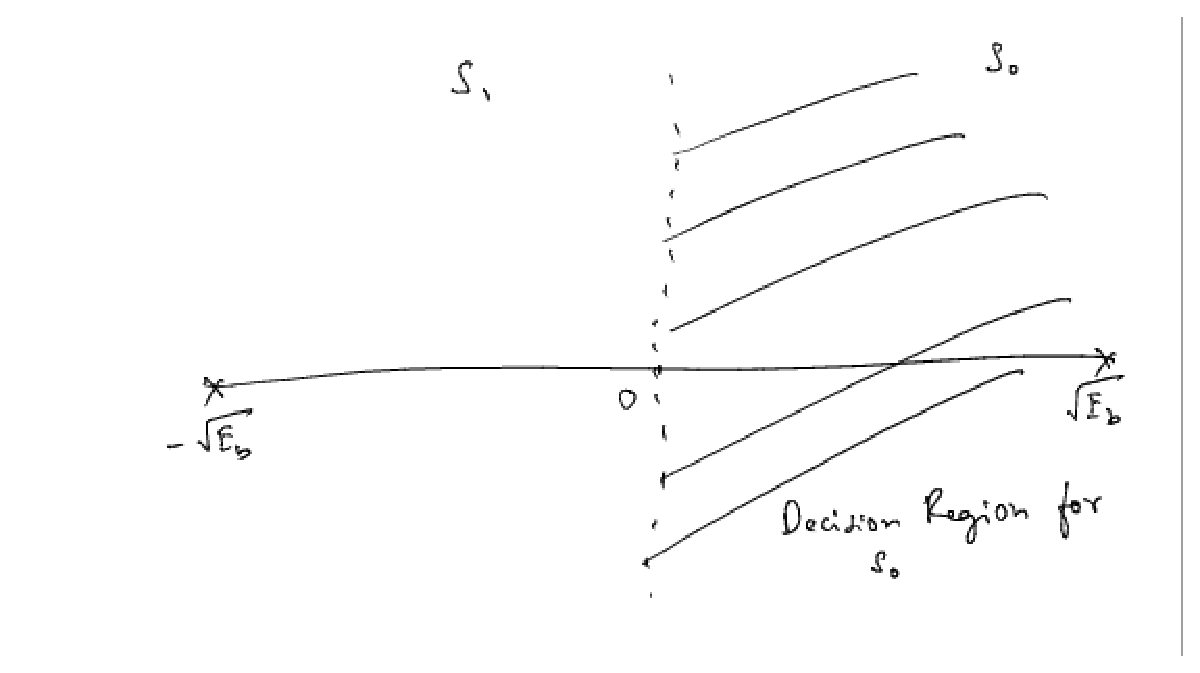
\includegraphics[width=\columnwidth]{./figs/bpsk_const.eps}
\caption{}
\label{fig:bpsk_const}
\end{figure}
\solution The possible received symbols are
\begin{align}
y|s_0 &= \sqrt{E_b} + n
\\
y|s_1 &= -\sqrt{E_b} + n
\end{align}
%
where the AWGN $n \sim \gauss{0}{\frac{N_0}{2}}$.
%
\begin{problem}
\label{prob:bpsk_decision}
From Fig. \ref{fig:bpsk_const} obtain a decision rule for BPSK
\end{problem}
\solution The decision rule is
\begin{equation}
y \dec{s_0}{s_1} 0
\end{equation}
\begin{problem}
Repeat the previous exercise using the MAP criterion.
\end{problem}
\begin{problem}
Using the decision rule in Problem \ref{prob:bpsk_decision}, obtain an expression for the probability of error for BPSK.
\end{problem}
\solution
Since the symbols are equiprobable, it is sufficient if the error is calculated assuming that a 0 was sent.  This results in
\begin{align}
P_e &= \pr{y < 0|s_0} = \pr{\sqrt{E_b} + n < 0}
\\
&= \pr{ -n > \sqrt{E_b} } = \pr{ n > \sqrt{E_b} }
\label{eq:bpsk_proof_n0}
\end{align}
since $n$ has a symmetric pdf.
Let $w \sim \gauss{0}{1}$.  Then $n = \sqrt{\frac{N_0}{2}}w$. Substituting this in \eqref{eq:bpsk_proof_n0},
\begin{align}
P_e &=  \pr{ \sqrt{\frac{N_0}{2}}w > \sqrt{E_b} } = \pr{ w > \sqrt{\frac{2E_b}{N_0}} }
\\
&= \qfunc{\sqrt{\frac{2E_b}{N_0}}}
\end{align}
%
where $\qfunc{x} \define \pr{w > x}, x \ge 0$.
\begin{problem}
The PDF of $w \sim \gauss{0}{1}$ is given by
%
\begin{equation}
p_{w}(x) = \frac{1}{\sqrt{2\pi}}\exp\brak{-\frac{x^2}{2}}, -\infty < x < \infty
\end{equation}
and the complementary error function is defined as
\begin{equation}
\operatorname {erfc} (x)={\frac {2}{\sqrt {\pi }}}\int _{x}^{\infty }e^{-t^{2}}\,dt.
\end{equation}
%
Show that 
\begin{equation}
Q(x) = \frac{1}{2}\operatorname {erfc}\left({\frac  {x}{{\sqrt  {2}}}}\right)
\end{equation}
\end{problem}
\begin{problem}
Verify the bit error rate (BER) plots for BPSK through simulation and analysis for 0 to 10 dB.
\end{problem}
\solution
The following code
\begin{lstlisting}
codes/bpsk_ber.py
\end{lstlisting}
yields Fig. \ref{fig:bpsk_ber}
\begin{figure}[!h]
\centering
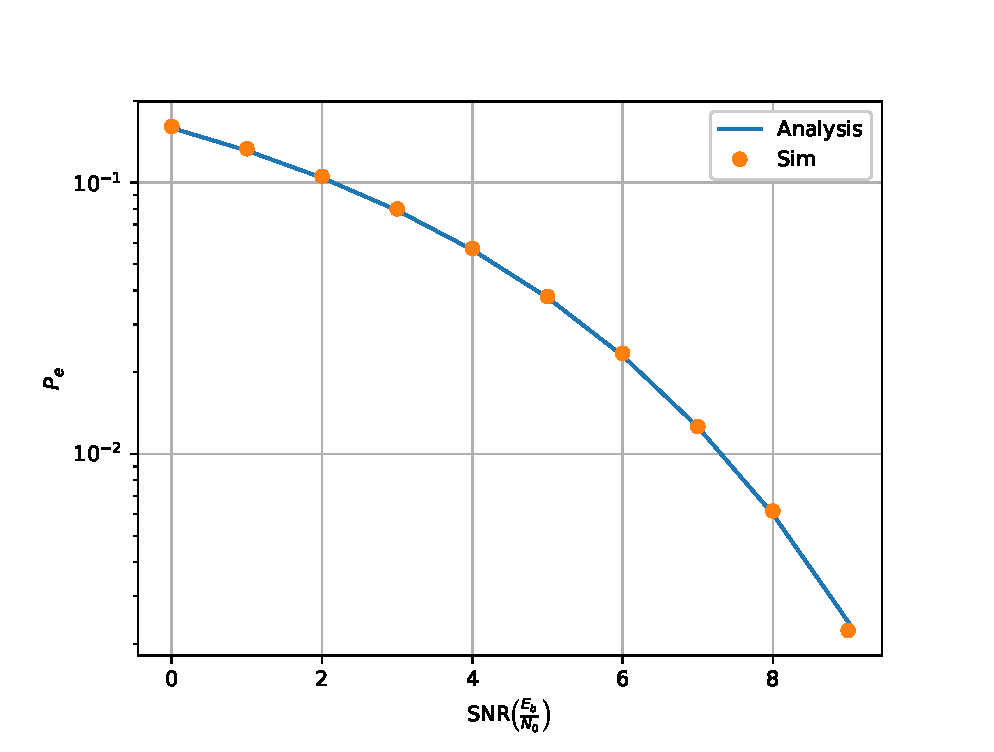
\includegraphics[width=\columnwidth]{./figs/bpsk_ber.eps}
\caption{}
\label{fig:bpsk_ber}
\end{figure}

\begin{problem}
Show that
\begin{equation}
Q(x) = \frac{1}{\pi}\int^{\frac{\pi}{2}}_{0}e^{-\frac{x^2}{2\sin^2 \theta}}\,d\theta
\end{equation}
\end{problem}
\section{Coherent BFSK}
\begin{problem}
The signal constellation for binary frequency shift keying (BFSK) is given in Fig. \ref{fig:bfsk_const}.
Obtain the equations for the received symbols.
\end{problem}
\begin{figure}[!h]
\centering
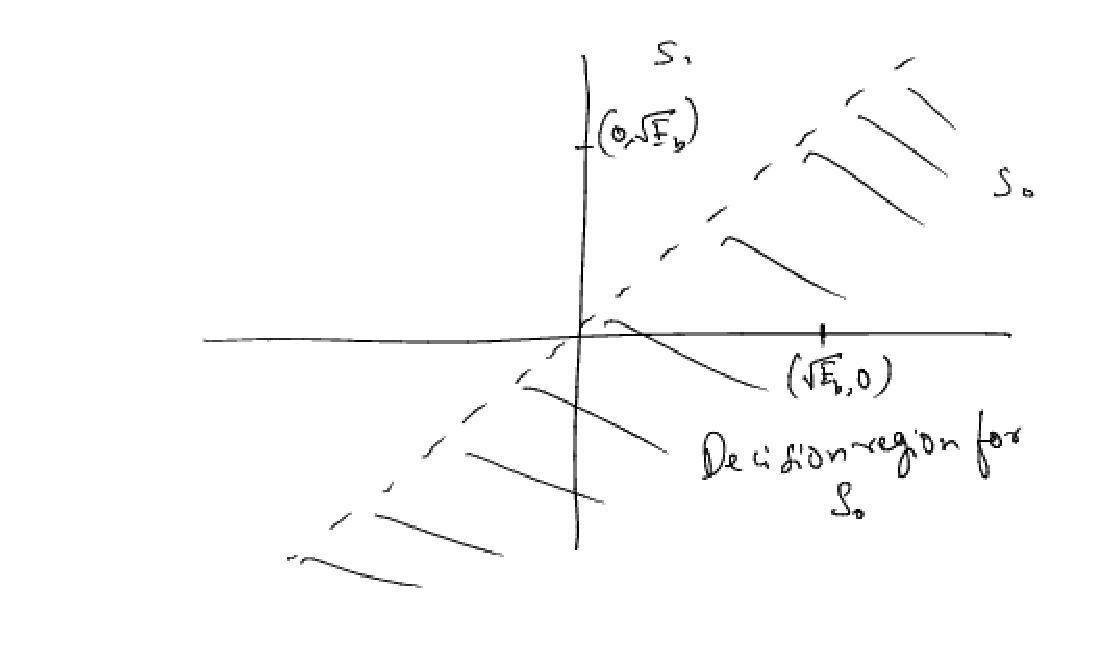
\includegraphics[width=\columnwidth]{./figs/bfsk_const.eps}
\caption{}
\label{fig:bfsk_const}
\end{figure}
\solution
The received symbols are given by
\begin{align}
\mathbf{y}|s_0 = 
\begin{pmatrix*}
\sqrt{E_b} \\
0
\end{pmatrix*}
+
\begin{pmatrix*}
 n_{1}\\
n_{2}
\end{pmatrix*},
\end{align}
and 
\begin{align}
\mathbf{y}|s_1 = 
\begin{pmatrix*}
0\\
\sqrt{E_b} 
\end{pmatrix*}
+
\begin{pmatrix*}
n_{1}\\
 n_{2}
\end{pmatrix*},
\end{align}
where $n_1,n_2 \sim \gauss{0}{\frac{N_0}{2}}$. and
$
\mathbf{y} = 
\begin{pmatrix*}
y_{1}\\
 y_{2}
\end{pmatrix*}
$.
\begin{problem}
Obtain a decision rule for BFSK from Fig. \ref{fig:bfsk_const}.
\end{problem}
\solution The decision rule is
\begin{equation}
\label{eq:bfsk_dec}
y_1 \dec{s_0}{s_1} y_2
\end{equation}
%The multivariate Gaussian distribution is defined as
%%
%\begin{multline}
%p_{\mathbf{x}}(x_1,\dots,x_k)
%\\
%=\frac{1}{\sqrt{\brak{2\pi}^k\abs{\Sigma}}}\exp\cbrak{-\frac{1}{2}\brak{\mathbf{x}-\mathbf{\mu}}^T\Sigma^{-1}\brak{\mathbf{x}-\mathbf{\mu}}}
%\end{multline}
%%
%where $\mathbf{\mu}$ is the mean vector, $\Sigma = E\sbrak{\brak{\mathbf{x}-\mathbf{\mu}}\brak{\mathbf{x}-\mathbf{\mu}}^T}$ is the covariance matrix and $\abs{\Sigma}$ is the determinant of $\Sigma$.
\begin{definition}
The joint PDF of $X,Y$ is given by
\begin{multline}
\label{eq:bivariate}
p(x,y)= \frac{1}{2\pi \sigma_x\sigma_y\sqrt{1-\rho^2}}\exp\lsbrak{-\frac{1}{2\brak{1-\rho^2}}}
\\
\times \rsbrak{\cbrak{\frac{\brak{x-\mu_x}^2}{\sigma_x^2}+\frac{\brak{y-\mu_y}^2}{\sigma_y^2}-\frac{2\rho\brak{x-\mu_x}\brak{y-\mu_y}}{\sigma_x\sigma_y}}}
\end{multline}
%
where
\begin{align}
\mu_x &= E\sbrak{X},
\sigma_x^2 = \text{var}\brak{X},
\rho = \frac{E\sbrak{\brak{X - \mu_x}\brak{Y-\mu_y}}}{\sigma_x\sigma_y}.
\end{align}
%where
%%
%\begin{align}
%\mathbf{\mu}=
%\begin{pmatrix*}
%\mu_x \\
%\mu_y
%\end{pmatrix*},
%\Sigma = 
%\begin{pmatrix*}%[r]
%\sigma_x^2 & \rho\sigma_x\sigma_y \\
%\rho\sigma_x\sigma_y & \sigma_y^2
%\end{pmatrix*}
%\end{align}
%
\end{definition}
%
\begin{problem}
For equiprobably symbols, the MAP criterion is defined as
%
\begin{equation}
\label{eq:map_bfsk_dec}
p\brak{\mathbf{y}|s_0} \dec{s_0}{s_1} p\brak{\mathbf{y}|s_1}
\end{equation}
Use \eqref{eq:bivariate} in \eqref{eq:map_bfsk_dec}  to obtain \eqref{eq:bfsk_dec}.
\end{problem}
\solution According to the MAP criterion, assuming equiprobably symbols,
\begin{align}
%\pr{ \mathbf{y}|s_0 }
p\brak{\mathbf{y}|s_0} \dec{s_0}{s_1} p\brak{\mathbf{y}|s_1}
\end{align}
\begin{problem}
Derive and plot the probability of error.  Verify through simulation.
\end{problem}
\solution Given that $s_0$ was transmitted, the received symbols are
\begin{align}
\mathbf{y}|s_0 = 
\begin{pmatrix*}
\sqrt{E_b} \\
0
\end{pmatrix*}
+
\begin{pmatrix*}
 n_{1}\\
n_{2}
\end{pmatrix*},
\end{align}
From \eqref{eq:bfsk_dec}, 
the probability of error is given by
\begin{align}
P_e &= \pr{y_1 < y_2|s_0} = \pr{\sqrt{E_b} + n_1 < n_2}
\\
&= \pr{ n_2-n_1 > \sqrt{E_b} } 
\label{eq:bfsk_proof_n0}
\end{align}
Note that $n_2-n_1 \sim \gauss{0}{N_0}$. Thus, 
\begin{align}
P_e &= \pr{ \sqrt{N_0}w > \sqrt{E_b} }  =  \pr{ w > \sqrt{\frac{E_b}{N_0}} }
%= \pr{ X > \sqrt{E_b} }
\\
\implies 
P_e & = \qfunc{\sqrt{\frac{E_b}{N_0}}}
\end{align}
where 
%$X \sim \gauss{0}{N_0}$
%\\
$w \sim \gauss{0}{1}$.  
%Then $X = \sqrt{N_0}w$. Substituting this in \eqref{eq:fsk_proof_n0},
%where $\qfunc{x} \define \pr{w > x}, x \ge 0$.
%
The following code plots the BER curves in Fig. \ref{fig:bfsk_ber}
\begin{lstlisting}
codes/fsk_ber.py
\end{lstlisting}
%
\begin{figure}[!h]
\centering
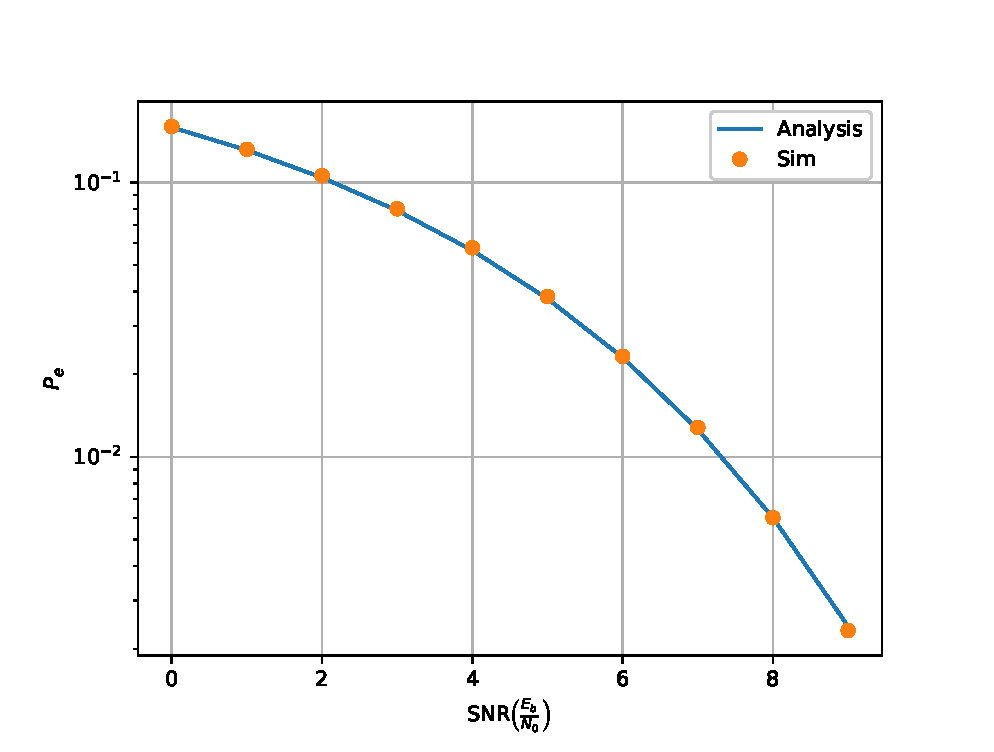
\includegraphics[width=\columnwidth]{./figs/bfsk_ber.eps}
\caption{}
\label{fig:bfsk_ber}
\end{figure}


\section{QPSK}
%\begin{problem}
Let
\begin{equation}
\mathbf{y} = \mathbf{s}+ \mathbf{n}
\end{equation}
where $\mathbf{s} \in \cbrak{\mathbf{s}_0,\mathbf{s}_1,\mathbf{s}_2, \mathbf{s}_3}$ and
\begin{align}
\mathbf{s}_0 &= 
\begin{pmatrix*}
\sqrt{E_s}\\
0
\end{pmatrix*},
\mathbf{s}_1 = 
\begin{pmatrix*}
0\\
\sqrt{E_s}
\end{pmatrix*},
\\
\mathbf{s}_2 &= 
\begin{pmatrix*}
-\sqrt{E_s}\\
0
\end{pmatrix*},
\mathbf{s}_3 = 
\begin{pmatrix*}
0\\
-\sqrt{E_s}
\end{pmatrix*},
\\
E\sbrak{\mathbf{n}} &= \mathbf{0}, E\sbrak{\mathbf{n}\mathbf{n}^T} = \sigma^2 \mathbf{I}
\end{align}
%
\begin{problem}
Show that the MAP decision for detecting $\mathbf{s}_0$ results in
\begin{equation}
\abs{y_2} < y_1
\end{equation}
\end{problem}
\begin{problem}
Express $\pr{\hat{\mathbf{s}} = \mathbf{s}_0|\mathbf{s} = \mathbf{s}_0}$ in terms of $r_1, r_2$.
Let $X=n_2-n_1, Y = -n_2-n_1$, where $\mathbf{n}=\brak{n_1,n_2}$.
Their correlation coefficient is defined as
%
\begin{align}
\rho = \frac{E\sbrak{\brak{X-\mu_x}\brak{Y-\mu_y}}}{\sigma_x\sigma_y}
\end{align}
%
$X$ and $Y$ are said to be uncorrelated if $\rho = 0$
\end{problem}
\begin{problem}
Show that if $X$ and $Y$ are uncorrelated 
Verify this numerically.
\end{problem}
\begin{problem}
Show that $X$ and $Y$ are independent, i.e. $p_{XY}(x,y) = p_{X}(x)p_{Y}(y)$.
\end{problem}
\begin{problem}
Show that $X,Y \sim \mathcal{N}\brak{0,N_0}$.
\end{problem}
\begin{problem}
Show that 
\begin{equation}
\pr{\hat{\mathbf{s}} = \mathbf{s}_0|\mathbf{s} = \mathbf{s}_0} =\pr{ X < \sqrt{E_s},  Y < \sqrt{E_s}}.
\end{equation}
\end{problem}
\begin{problem}
Show that 
\begin{equation}
\pr{ X < \sqrt{E_s},  Y < \sqrt{E_s}} = \brak{1-\qfunc{\sqrt{\frac{E_s}{N_0}}}}^2
\end{equation}
\end{problem}
\begin{problem}
Verify the above through simulation.
\end{problem}
\solution 
This is shown in Fig. \ref{fig:qpsk} through the following code.
\begin{lstlisting}
codes/qpsk.py
\end{lstlisting}
%
\begin{figure}[!h]
\centering
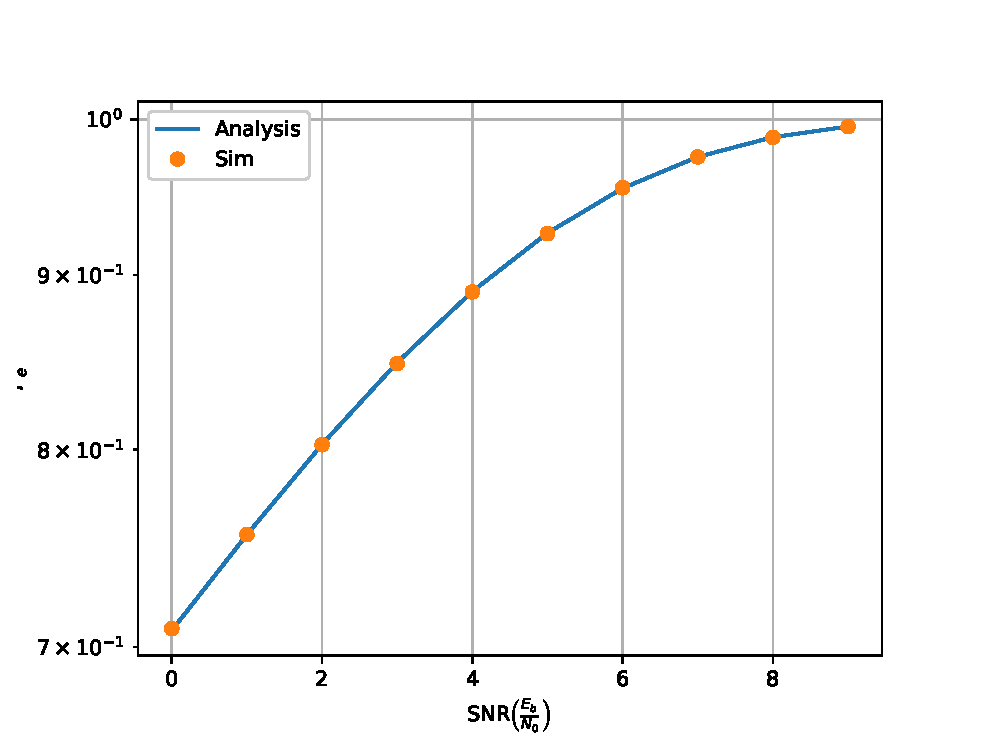
\includegraphics[width=\columnwidth]{./figs/qpsk.eps}
\caption{}
\label{fig:qpsk}
\end{figure}
\begin{problem}
Modify the above script to obtain the probability of symbol error.
\end{problem}

%\begin{enumerate}
%\item 
%\item 
%\item 
%\item 
%\item 
%\item 
%\\
%\solution Given we transmitted $s_0$, the probability of decoding it as $s_0$ is given by 
%\begin{equation}
%\pr{\hat{\mathbf{s}} = \mathbf{s}_0|\mathbf{s} = \mathbf{s}_0} = \pr{-n_2<\sqrt{E_s}+n_1,\sqrt{E_s}+n_1>n_2} 
%\end{equation}
%\begin{equation}
%\implies \pr{\hat{\mathbf{s}} = \mathbf{s}_0|\mathbf{s} = \mathbf{s}_0} = \pr{X<\sqrt{E_s},Y<\sqrt{E_s}}
%\end{equation}
%\\
%Where, $X=n_2-n_1, Y=-n_2-n_1$. Also $X,Y \sim \mathcal{N}\brak{0,2\sigma^2}$ and are independent. 
%\item Show that 
%\begin{equation}
%\pr{ X < \sqrt{E_s},  Y < \sqrt{E_s}} = \brak{1-\qfunc{\sqrt{\frac{E_s}{N_0}}}}^2
%\end{equation}
%\solution 
%\begin{equation}
%\pr{X < A, Y < A} = \pr{X < A}\pr{Y < A}
%\end{equation}
%\begin{equation}
%\implies \pr{X < A, Y < A} = \brak{1-\qfunc{\frac{A}{\sqrt{2}\sigma}}}^2
%\end{equation}
%\item 
%\\
%
%\item 
%\end{enumerate}
%\end{problem}
\section{$M$-PSK}

Consider a system where 
$\mathbf{s}_i=
\begin{pmatrix}
\cos\brak{\frac{2\pi i}{M}}\\
\cos\brak{\frac{2\pi i}{M}}
\end{pmatrix}, i = 0, 1 , \dots M-1
$
.
Let
%
\begin{align}
\mathbf{y}|s_0 = 
\begin{pmatrix}
y_1\\
y_2
\end{pmatrix}
=
\begin{pmatrix}
\sqrt{E_s}+n_1\\
n_2
\end{pmatrix}
\end{align}
where $n_1,n_2 \sim \mathcal{N}\brak{0,\frac{N_0}{2}}$.
\begin{problem}
 Substituting 
\begin{align}
y_1=R\cos \theta \\
y_2=R\sin \theta
\end{align}
show that the joint pdf of $R,\theta$ is
%
\begin{equation}
p\brak{R,\theta}=\frac{R}{\pi N_0}\exp\brak{-\frac{R^2-2R\sqrt{E_s}\cos \theta + E_s}{N_0}}
\end{equation}
\end{problem}
\begin{problem}
Show that 
%
\begin{align}
\lim_{\alpha \rightarrow \infty}\int_{0}^{\infty}\brak{V-\alpha }e^{-\brak{V-\alpha}^2 }\,dV
&= 0
\\
\lim_{\alpha \rightarrow \infty}\int_{0}^{\infty} e^{-\brak{V-\alpha}^2 }\,dV
&=  \sqrt{\pi}
\end{align}
\end{problem}
\begin{problem}
Using the above, show that
%
\begin{multline}
\int_{0}^{\infty}V\exp\cbrak{-\brak{V^2 - 2V \sqrt{\gamma}\cos \theta +\gamma}}\,dV
\\
= e^{-\gamma\sin^2 \theta} \sqrt{\gamma\pi}\cos \theta
\end{multline}
%
for large values of $\gamma$.
\end{problem}
\begin{problem}
Find a compact expression for
%
\begin{align}
I = 1 - \sqrt{\frac{\gamma}{\pi}}\int_{-\frac{\pi}{M}}^{\frac{\pi}{M}}e^{- \gamma\sin^2\theta }\cos \theta\, d\theta
\end{align}
\end{problem}
\begin{problem}
Show that
\begin{equation}
P_{e|\mathbf{s}_0}=2\qfunc{\sqrt{2\brak{\frac{{E_s}}{N_o}}}\sin \frac{\pi}{M}}
\end{equation}
\end{problem}
\begin{problem}
Verify the SER through simulation.
\end{problem}

%
\end{document}


